%\includegraphics[width=\linewidth]{salome_architecture.pdf}
\documentclass[tikz,border=3pt]{standalone}
\usepackage[T1]{fontenc}
\usepackage{lmodern}
\usepackage{fontawesome5} % scalable vector Python logo
\renewcommand{\familydefault}{\sfdefault}
\usetikzlibrary{arrows.meta,calc,shapes.geometric,positioning}
\definecolor{navy}{RGB}{25,48,86}
\definecolor{sky}{RGB}{30,158,216}
\definecolor{pale}{RGB}{237,249,255}
\definecolor{steel}{RGB}{117,132,145}
\definecolor{bluearrow}{RGB}{44,125,206}
\tikzset{every node/.style={font=\sffamily},arr/.style={-{Triangle[length=4.2mm,width=3.7mm]},line width=1.6pt,draw=navy},both/.style={{Triangle[length=3.7mm,width=3mm]}-{Triangle[length=3.7mm,width=3mm]},line width=1.7pt,draw=bluearrow}}
\newcommand{\cuboid}[4]{% x,y,width,label; fixed height 2.49
  \path[fill=gray!41,draw=gray!65,line width=.4pt] (#1,#2) rectangle ++(#3,2.49);
  \path[fill=gray!24,draw=gray!62,line width=.4pt] (#1,#2+2.49) -- ++(.31,.30) -- ++(#3,0) -- ++(-.31,-.30) -- cycle;
  \path[fill=gray!58,draw=gray!65,line width=.4pt] (#1+#3,#2) -- ++(.31,.30) -- ++(0,2.49) -- ++(-.31,-.30) -- cycle;
  \node[anchor=north,align=center,text=black,font=\sffamily\bfseries\fontsize{9.5}{11}\selectfont] at (#1+#3/2,#2+2.19) {#4};
}
\newcommand{\barblock}[5]{% x y width height title
 \path[fill=#5,draw=gray!60,line width=.45pt] (#1,#2) rectangle ++(#3,#4);
 \path[fill=gray!30,draw=gray!60,line width=.45pt] (#1,#2+#4) -- ++(.28,.18) -- ++(#3,0) -- ++(-.28,-.18) -- cycle;
 \path[fill=gray!72,draw=gray!60,line width=.45pt] (#1+#3,#2) -- ++(.28,.18) -- ++(0,#4) -- ++(-.28,-.18) -- cycle;
}
\begin{document}
\begin{tikzpicture}[x=1cm,y=1cm,line cap=round,line join=round]
% Background and system boundaries
\path[fill=white] (0,0) rectangle (16,12);
% Two external panels
\foreach \xa/\xb/\title in {1.53/7.27/External Files,8.83/15.35/External Solvers}{
 \path[rounded corners=2.2mm,fill=white,draw=navy,line width=.75pt] (\xa,9.58) rectangle (\xb,11.86);
 \path[rounded corners=2.2mm,fill=navy] (\xa,11.32) rectangle (\xb,11.86);
 \path[fill=navy] (\xa,11.32) rectangle (\xb,11.61);
 \node[text=white,font=\bfseries\fontsize{15}{17}\selectfont] at ({(\xa+\xb)/2},11.57) {\title};
}
% External CAD document icon
\begin{scope}[shift={(2.63,10.2)}]
 \path[draw=black,fill=gray!9,line width=.8pt] (0,0) -- (0,1) -- (.62,1) -- (.82,.79) -- (.82,0) -- cycle;
 \path[draw=black,fill=gray!24] (.62,1)--(.62,.79)--(.82,.79);
 \draw[line width=.65pt] (.12,.58)--(.32,.7)--(.52,.58)--(.32,.46)--cycle;
 \draw[line width=.65pt] (.32,.7)--(.32,.46) (.52,.58)--(.52,.34)--(.32,.21)--(.12,.34)--(.12,.58);
 \draw[line width=.65pt] (.12,.34)--(.32,.46)--(.52,.34);
\end{scope}
\node[font=\bfseries\fontsize{10}{11}\selectfont] at (3.04,9.78) {CAD Files};
% External mesh file icon
\begin{scope}[shift={(5.12,10.2)}]
 \path[draw=black,fill=gray!9,line width=.8pt] (0,0) -- (0,1) -- (.61,1) -- (.83,.77) -- (.83,0) -- cycle;
 \path[draw=black,fill=gray!23] (.61,1)--(.61,.77)--(.83,.77);
 \draw[line width=.55pt] (.12,.17)--(.32,.76)--(.68,.49)--(.55,.16)--cycle (.12,.17)--(.68,.49) (.32,.76)--(.55,.16);
\end{scope}
\node[font=\bfseries\fontsize{10}{11}\selectfont] at (5.54,9.78) {Mesh Files};
% External solvers: editable vector server symbols
\foreach \x/\name in {9.39/1,11.25/2,14.16/N}{
 \begin{scope}[shift={(\x,10.18)}]
 \path[fill=gray!19,draw=black,line width=.6pt] (0,0) rectangle (.43,.95);
 \path[fill=gray!43,draw=black,line width=.6pt] (.43,0)--(.59,.17)--(.59,1.12)--(.43,.95)--cycle;
 \path[fill=gray!8,draw=black,line width=.6pt] (0,.95)--(.16,1.12)--(.59,1.12)--(.43,.95)--cycle;
 \foreach \j in {.19,.30,.41,.52,.63,.74}{\draw[gray!70,line width=.5pt] (.11,\j)--(.33,\j);}
 \draw[fill=blue!25,draw=navy,line width=.55pt] (.51,.12) circle (.14);
 \draw[fill=gray!8,draw=navy,line width=.45pt] (.51,.12) circle (.055);
 \end{scope}
 \node[font=\bfseries\fontsize{9.5}{10}\selectfont] at (\x+.26,9.78) {Solver \name};
}
\node[font=\bfseries\large] at (13.2,10.65) {$\cdots$};
% SALOME platform panel styled like the external blocks without the blue background
\path[rounded corners=2.2mm,fill=white,draw=navy,line width=.75pt] (.25,2.60) rectangle (15.75,8.86);
\path[rounded corners=2.2mm,fill=navy] (.25,8.20) rectangle (15.75,8.86);
\path[fill=navy] (.25,8.20) rectangle (15.75,8.56);
\node[text=white,font=\bfseries\fontsize{15}{17}\selectfont] at (7.0,8.49) {SALOME};
% All module cuboids (equal grey) and shared service layers
\barblock{.5}{3.84}{14.76}{.73}{black!30}
\barblock{.5}{2.91}{14.76}{.73}{black!30}
\node[font=\bfseries\fontsize{9}{9}\selectfont,text=magenta] at (7.97,4.20) {KERNEL};
\node[font=\bfseries\fontsize{9}{9}\selectfont,text=magenta] at (7.97,3.28) {GUI};
\cuboid{.72}{4.69}{2.64}{Geometry}
\node[font=\bfseries\fontsize{7}{7}\selectfont,text=magenta] at (1.99,4.92) {GEOM{\color{black},} SHAPER};
\cuboid{3.52}{4.69}{2.64}{Meshing}
\node[font=\bfseries\fontsize{7}{7}\selectfont,text=magenta] at (4.79,4.92) {SMESH{\color{black},} HOMARD};

\cuboid{6.32}{4.69}{3.03}{Code Supervision\\\& Coupling}
\node[font=\bfseries\fontsize{7}{7}\selectfont,text=magenta] at (7.79,4.92) {YACS{\color{black},} EFICAS{\color{black},} ...};

\cuboid{9.51}{4.69}{2.68}{Visualization}
\node[font=\bfseries\fontsize{7}{7}\selectfont,text=magenta] at (10.99,4.92) {PARAVIS};


\cuboid{12.35}{4.69}{2.64}{Uncertainty\\Quantification}
\node[font=\bfseries\fontsize{7}{7}\selectfont,text=magenta] at (13.79,4.92) {PERSALYS};

% Geometry cube icon
\begin{scope}[shift={(1.66,5.23)},scale=.80]
 \path[draw=black,fill=white,line width=.9pt] (0,0)--(.71,0)--(.71,.73)--(0,.73)--cycle;
 \path[draw=black,fill=gray!25,line width=.9pt] (.71,0)--(1.02,.28)--(1.02,1.01)--(.71,.73)--cycle;
 \path[draw=black,fill=gray!7,line width=.9pt] (0,.73)--(.31,1.01)--(1.02,1.01)--(.71,.73)--cycle;
\end{scope}
% Mesh wireframe 3D polyhedron
\begin{scope}[shift={(4.36,5.24)},scale=.80]
 \coordinate (a) at (0,.18);\coordinate (b) at (.48,1.18);\coordinate (c) at (1.15,.83);\coordinate (d) at (1.12,.05);\coordinate (e) at (.39,-.06);\coordinate (f) at (.65,.55);
 \draw[line width=.9pt] (a)--(b)--(c)--(d)--(e)--cycle (a)--(f)--(b) (f)--(c) (f)--(d) (f)--(e) (b)--(d) (a)--(c);
\end{scope}
% Coupling icon: interlocking schematic plugs/puzzle pieces
\begin{scope}[shift={(7.13,5.00)}]
 \path[draw=navy,fill=blue!62,line width=.8pt] (0,.16)--(.36,.16)--(.36,.38) arc[start angle=180,end angle=0,radius=.14] --(.64,.16)--(.82,.16)--(.82,.64)--(.61,.64) arc[start angle=-90,end angle=-270,radius=.12] --(.82,.88)--(.36,.88)--(.36,.64)--(0,.64)--cycle;
 \path[draw=navy,fill=white,line width=.8pt] (.82,.16)--(1.32,.16)--(1.32,.37) arc[start angle=180,end angle=0,radius=.12]--(1.56,.16)--(1.62,.16)--(1.62,.88)--(1.38,.88) arc[start angle=0,end angle=180,radius=.12]--(1.14,.88)--(.82,.88)--(.82,.64)--(.82,.16)--cycle;
\end{scope}
% Visualization monitor and editable contour ellipses
\begin{scope}[shift={(10.40,5.12)},scale=.80]
 \path[draw=black,fill=black!85,rounded corners=.8mm,line width=.6pt] (0,.26) rectangle (1.34,1.15);
 \path[draw=black,fill=cyan!28] (.08,.36) rectangle (1.26,1.07);
 \begin{scope}
 \clip (.08,.36) rectangle (1.26,1.07);
 \draw[blue!80!black,line width=13pt,rotate around={25:(.67,.7)}] (.35,.7) ellipse (.43 and .09);
 \draw[cyan,line width=10pt,rotate around={25:(.67,.7)}] (.35,.7) ellipse (.43 and .09);
 \draw[green!80!yellow,line width=6pt,rotate around={25:(.67,.7)}] (.35,.7) ellipse (.43 and .09);
 \draw[yellow,line width=3pt,rotate around={25:(.67,.7)}] (.35,.7) ellipse (.43 and .09);
 \draw[red,line width=1.2pt,rotate around={25:(.67,.7)}] (.35,.7) ellipse (.43 and .09);
 \end{scope}
 \draw[draw=black,line width=2pt] (.67,.26)--(.67,.04) (.43,.04)--(.91,.04);
\end{scope}
% Uncertainty curves (normal distribution icons)
\begin{scope}[shift={(13.21,5.22)},scale=.70]
 \draw[black,line width=.65pt,-{Stealth[length=2mm]}] (0,0)--(1.35,0);
 \draw[black,line width=.65pt,-{Stealth[length=2mm]}] (0,0)--(0,1.1);
 \path[fill=violet!24] plot[smooth] coordinates {(.06,0) (.18,.03) (.36,.30) (.53,.93) (.68,.31) (.86,.03) (1.2,0)} -- cycle;
 \path[fill=blue!12] plot[smooth] coordinates {(.08,0) (.24,.08) (.46,.5) (.69,.69) (.91,.45) (1.17,.04) (1.29,0)} -- cycle;
 \draw[violet!70!black,line width=.9pt] plot[smooth] coordinates {(.06,0) (.18,.03) (.36,.30) (.53,.93) (.68,.31) (.86,.03) (1.2,0)};
 \draw[navy,line width=.9pt] plot[smooth] coordinates {(.08,0) (.24,.08) (.46,.5) (.69,.69) (.91,.45) (1.17,.04) (1.29,0)};
\end{scope}
% Input-output connections: CAD + mesh import arrows, bidirectional solver coupling
\draw[arr,color=bluearrow] (3.03,9.56)--(3.03,7.57);
\draw[arr,color=bluearrow] (5.53,9.56)--(5.53,7.57);
\draw[both] (8.95,9.56)--(8.95,7.57);
% User interaction panel styled like the external blocks without the blue background
\path[rounded corners=2.2mm,fill=white,draw=navy,line width=.75pt] (.25,.01) rectangle (15.75,2.00);
\path[rounded corners=2.2mm,fill=navy] (.25,2.12) rectangle (15.75,1.59);
%\path[fill=navy] (.25,2.52) rectangle (15.75,2.88);
\node[text=white,font=\bfseries\fontsize{15}{17}\selectfont] at (10.0,1.85) {User Interaction};
% GUI display
\begin{scope}[shift={(2.33,0.46)},scale=.68]
 \path[draw=black,fill=gray!35,rounded corners=.7mm] (0,.25) rectangle (1.06,1.05);
 \path[draw=black,fill=white] (.08,.34) rectangle (.98,.97);
 \foreach \xx/\yy/\cc in {.11/.67/red!75,.55/.67/green!70,.11/.38/cyan!60,.55/.38/violet!60}{\path[fill=\cc] (\xx,\yy) rectangle ++(.40,.26);}
 \draw[line width=1.3pt] (.53,.25)--(.53,.09) (.30,.09)--(.77,.09);
\end{scope}
\node[font=\bfseries\fontsize{10}{11}\selectfont] at (2.76,.18) {GUI};
% TUI terminal
\begin{scope}[shift={(6.9,0.49)},scale=.78]
 \path[fill=black!85,rounded corners=1mm,draw=gray!65,line width=.9pt] (0,0) rectangle (1.06,.85);
 \node[white,font=\ttfamily\fontsize{19}{20}\selectfont] at (.53,.43) {>\_};
\end{scope}
\node[font=\bfseries\fontsize{10}{11}\selectfont] at (7.31,.18) {CLI};
% Python icon: recognizable Font Awesome Python snake silhouette in its two brand colors.
% The glyph stays vector; each copy is clipped to show one colored half.
\begin{scope}[shift={(12.00,0.46)},scale=.78]
  \begin{scope}
    \clip (-.01,.43) rectangle (1.91,1.09);
    \node[anchor=south west,inner sep=0,outer sep=0,text={rgb,255:red,48;green,105;blue,152},font=\fontsize{23}{23}\selectfont] at (0,0) {\faPython};
  \end{scope}
  \begin{scope}
    \clip (-.04,-.02) rectangle (1.91,.43);
    \node[anchor=south west,inner sep=0,outer sep=0,text={rgb,255:red,255;green,208;blue,65},font=\fontsize{23}{23}\selectfont] at (0,0) {\faPython};
  \end{scope}
\end{scope}
\node[font=\bfseries\fontsize{10}{11}\selectfont] at (12.58,.18) {Python Scripting};
% User / platform exchange arrow
\draw[both] (2.69,1.18)--(2.69,2.62);
\draw[both] (12.29,1.18)--(12.29,2.62);
\draw[both] (7.29,1.18)--(7.29,2.62);
\end{tikzpicture}
\end{document}
